\section{Integrationstest}
Ved integrationstesten samkobles alt hardware. Integrationstesten er alle modultests samlet under en. 

\subsection{Opstilling og forbindelser}
Hardwaren er afhængig af: +-12V, 5V, Fælles ground og 18Vac/50Hz. Desuden skal STK500 kittet DE2boarded forsynes med spænding fra deres tilhørende 230V transformere. Ved 18Vac/50Hz spændingskilden benyttes den tilgængelige 230V transformer. 

Enkoderen skal forsynes med 5V, dette gøres direkte fra labratorietsforsyning.
Decoderen indeholder en operationsforstærker, hvis forsyning skal være +- 12V. Resten af decoderen skal forsynes med 5V. Dette gøres via en spændingsregulator på decoder printet.   

\begin{figure}[htb]
  \begin{minipage}{0.45\textwidth}
    \centering
      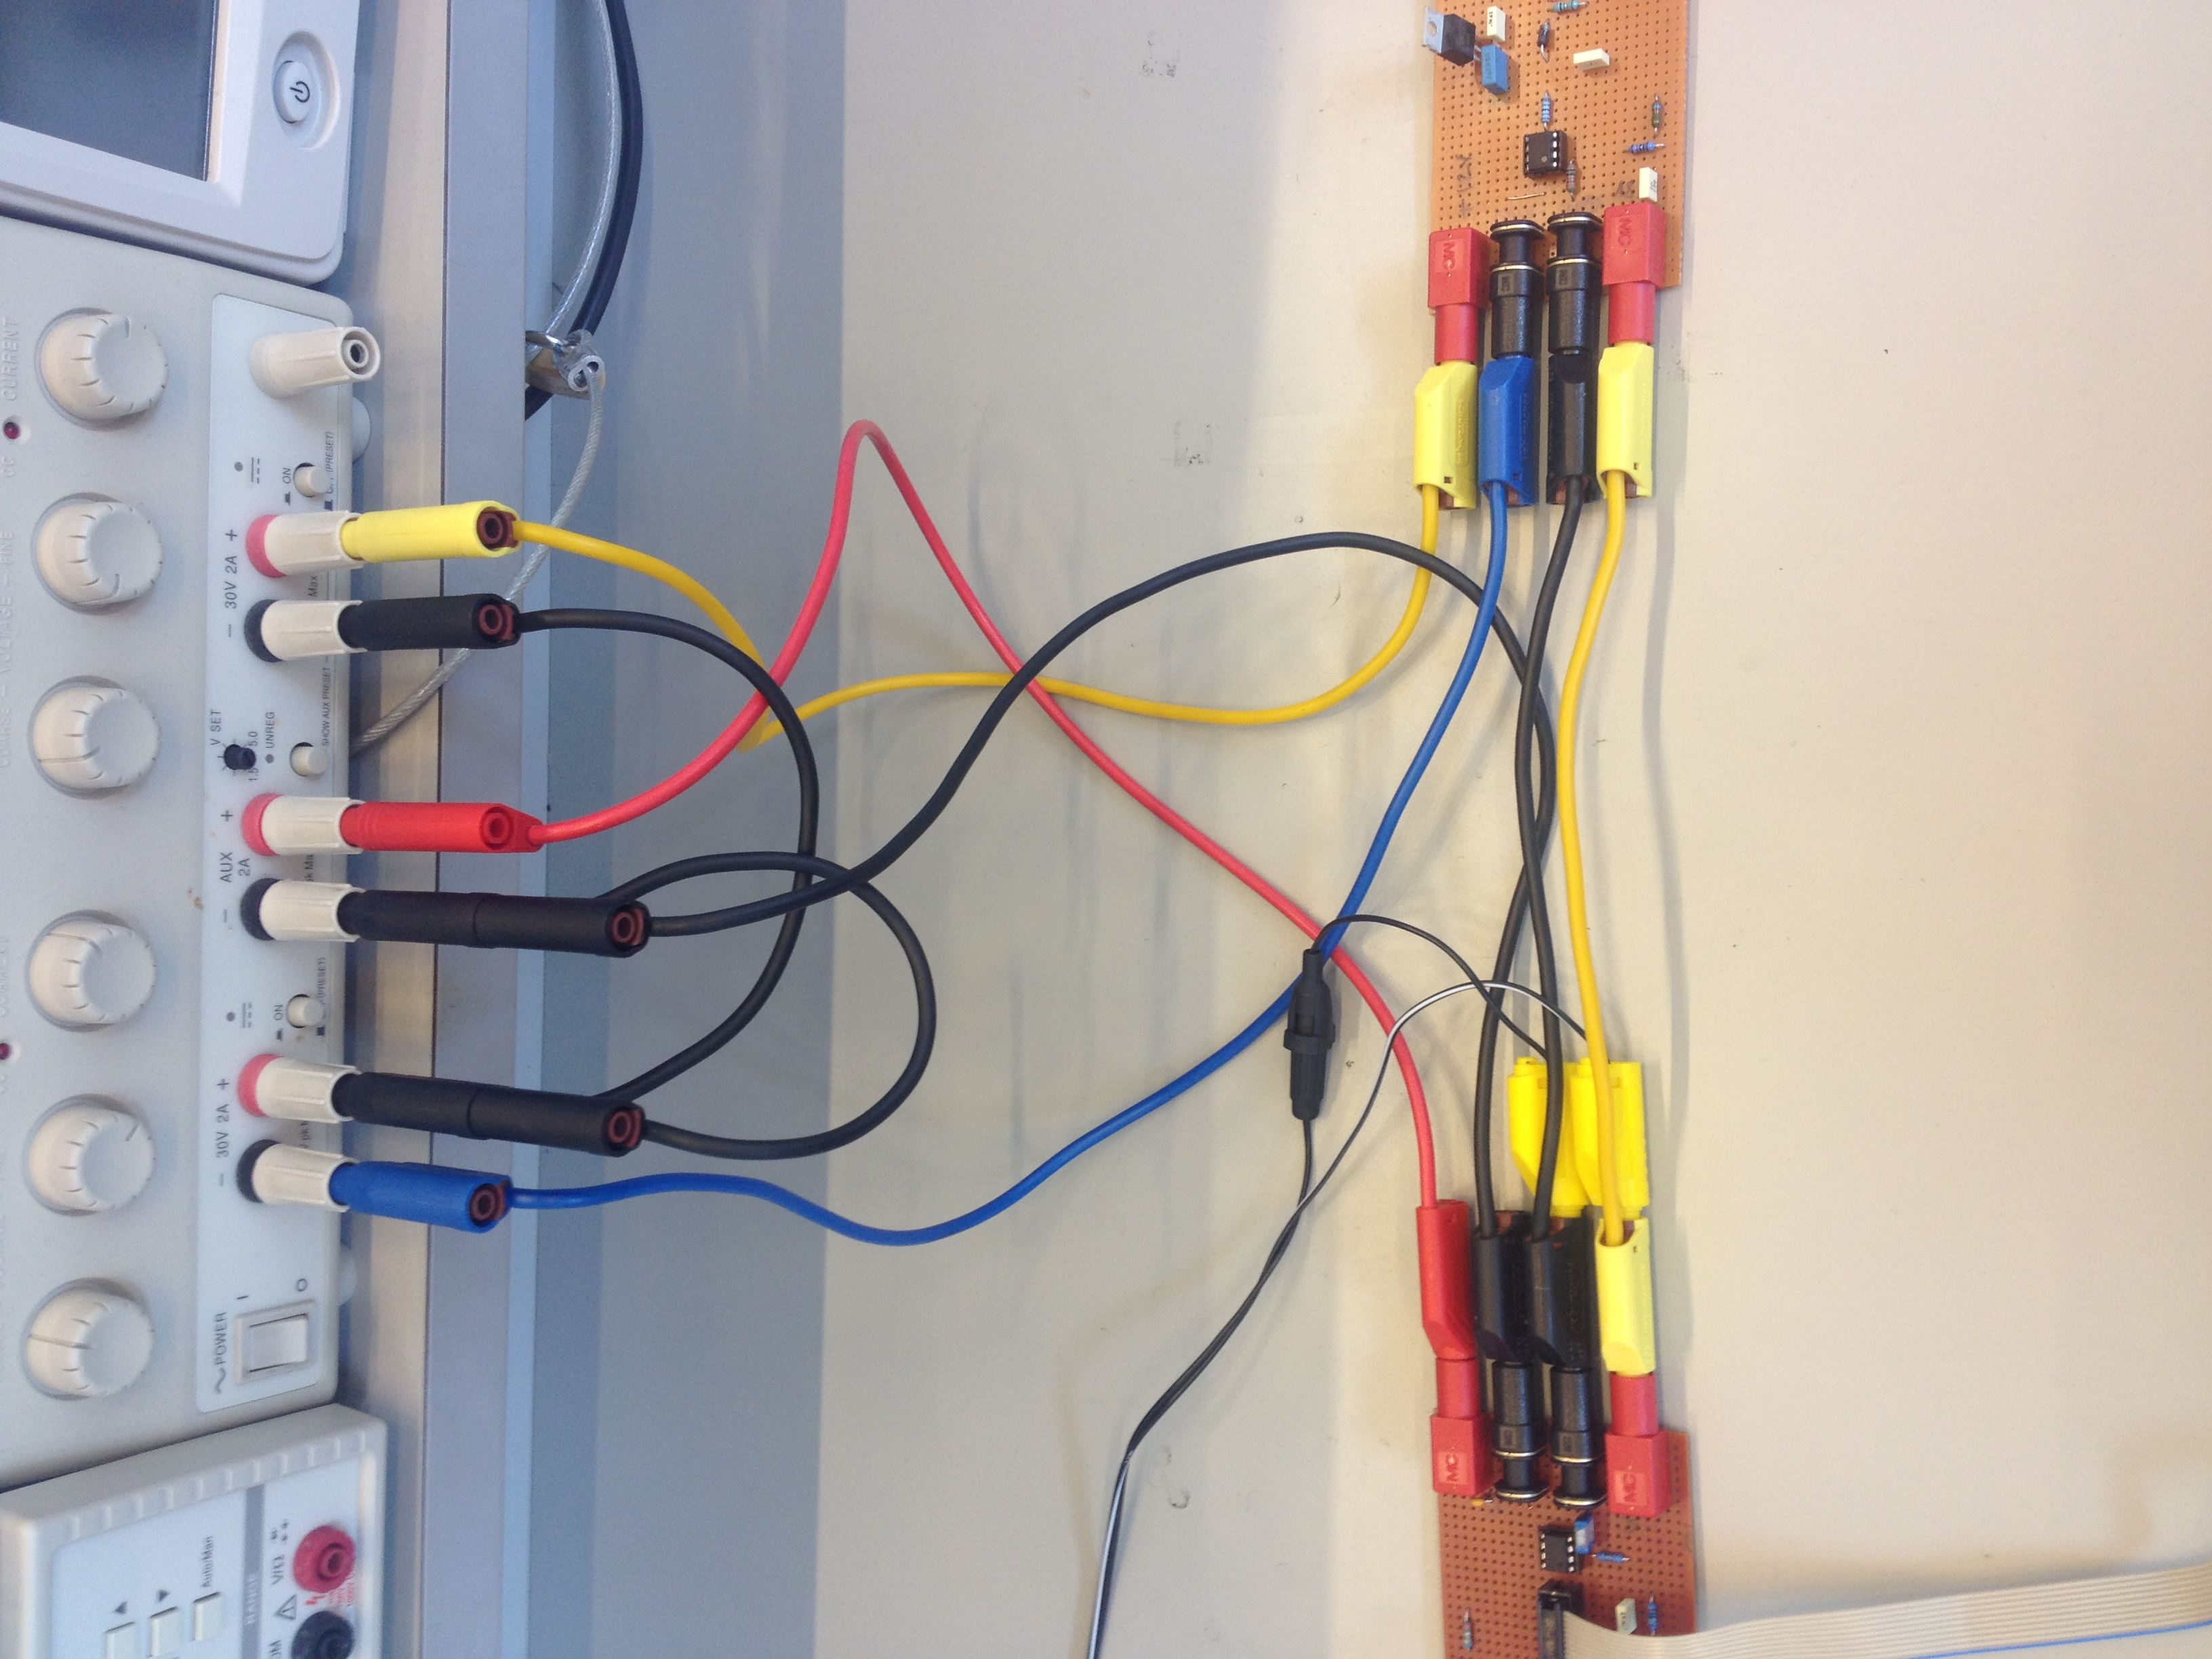
\includegraphics[width=\textwidth]{billeder/IntTest/forsyning}
      \caption{Opkobling af forsyning}
    \label{fig:opkobling_forsyning}
  \end{minipage}
  \hspace{0.1\textwidth}
  \begin{minipage}{0.45\textwidth}
    \centering
      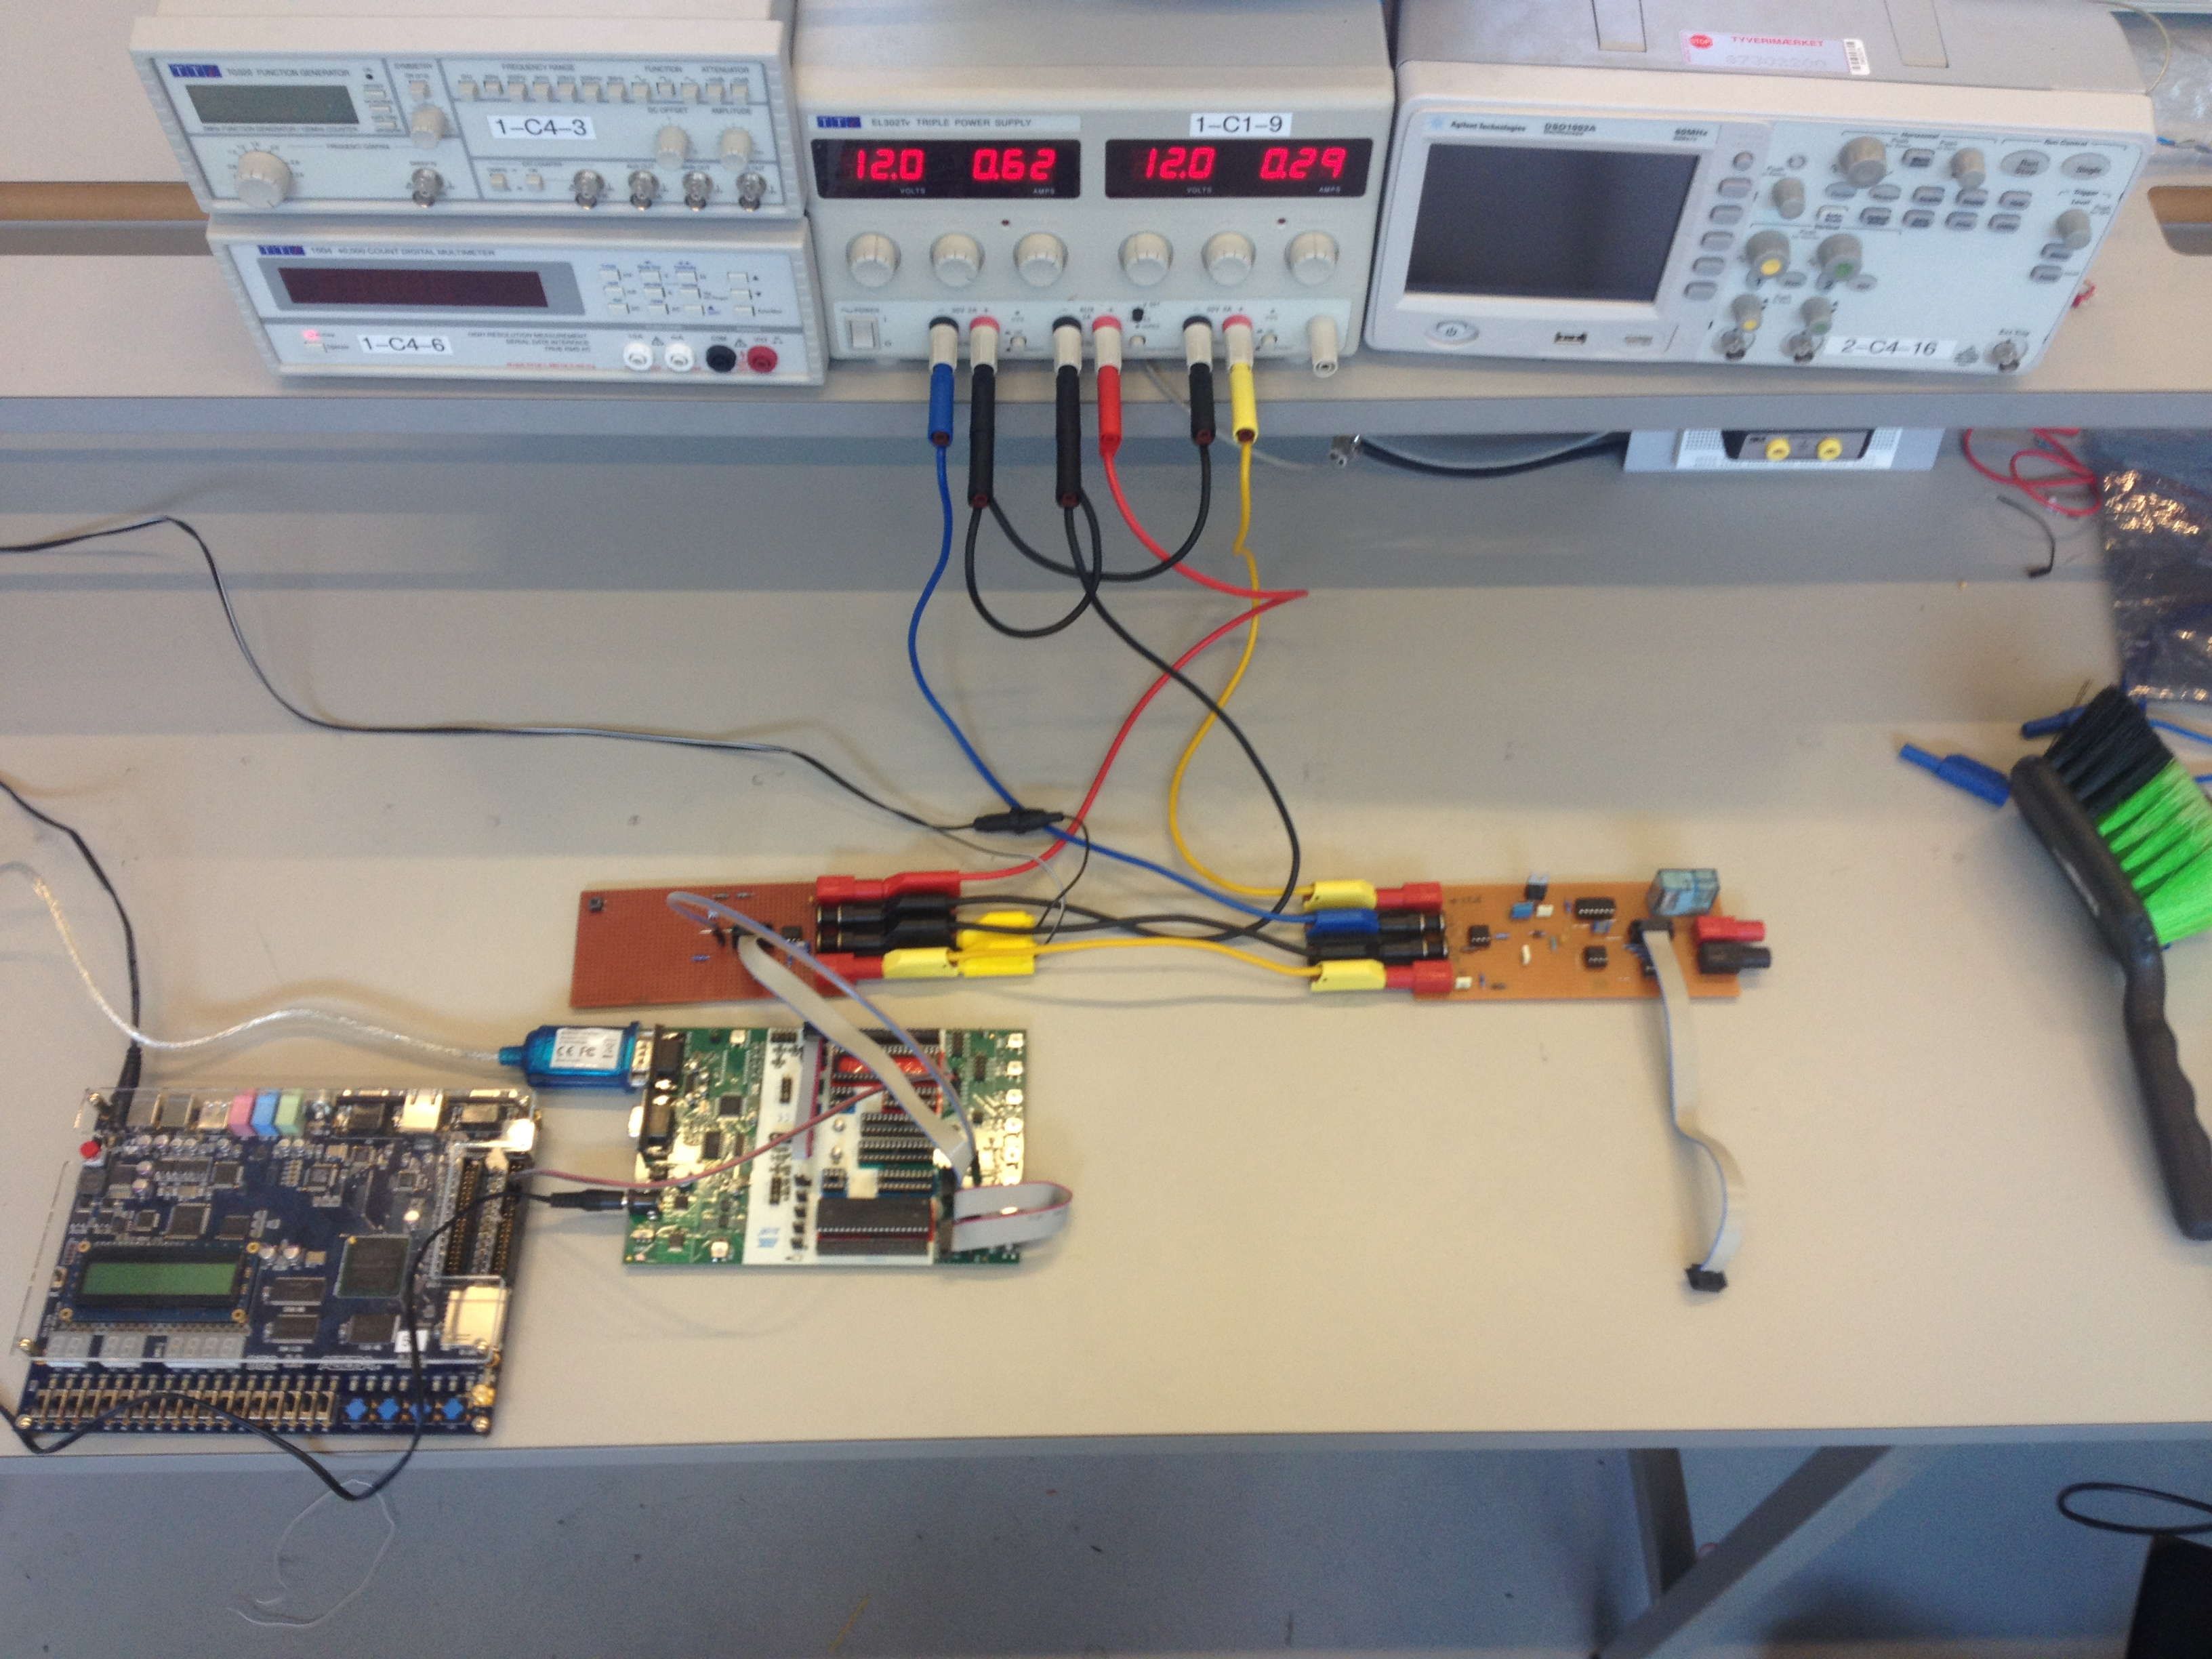
\includegraphics[width=\textwidth]{billeder/IntTest/system}
      \caption{Overbliksbillede af samlet opsætning}
    \label{fig:system_sammensat}
  \end{minipage}
\end{figure}

Spændingsforsyningen i labratoriet har 2 variable udgange (én til venstre og én til højre), samt én fast 5 V forsyning (midten). Begge variable udgange indstilles til 12V. 
Som det ses af \ref{fig:opkobling_forsyning} er + udgangen af udgangen til venstre kortsluttet med - udgangen af udgangen til højre. Dette skaber et 0 punkt, fællesground. Herved opnås -12V i den venstre -udgang, samt +12V i den højre + udgang. 0 punktet forbindes til - udgangen på den faste 5V forsyning, for at skabe fælles ground på hele forsyningen. På encoderprintet er der skabt fællesground mellem forsyningen og 18Vac/50Hz.

Encoderen tilsluttes +5V og ground.
Decoderen tilsluttes +-12V.

18Vac/50Hz skaber forbindelse mellem encoder og decoder.

Hovedenhedens STK500 kit tilsluttes PC'en via RS232 til USB. For at PC'en kan kommunikere med mikrocontrolleren skal PD0 tilsluttes RDX pinnen på STK500 og PD1 skal tilsluttes TDX pinnen på STK500. 

Hele port D fra STK500 kittet overføres til encoder printet. Yderligere information omkring forbinderserne i port D findes i hardwadre design for encoderen ***HENVISNING***

DE2 forbindelsen til STK500 *****

\subsection{Resultat}


\begin{figure}[htbp]
	\centering
	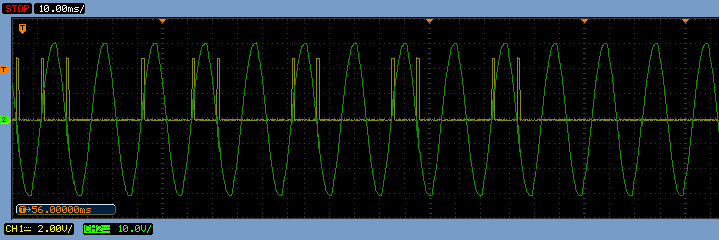
\includegraphics[width=\textwidth]{billeder/IntTest/Modtager_0101_ON}
	\caption{.}
	\label{fig:Modtager_0101_ON}
\end{figure}

Ovenstående \ref{fig:Modtager_0101_ON} viser hvad decoderen ville sende til modtager STK500 kittet, hvis dette var implementeret. Fra PC'en er kommandoen for at aktivere udtag med adresse "0101" sendt afsted.
"1110 0101100110 01100110 000000" er den modtagede X10 kode, netop den kode som aktiverer udtaget med adresse "0101". Det er her op til modtager softwaren at arbejde med denne kode og herved sætte PD7 høj. Herved vil relæet klikke og 18Vac/50Hz udtaget er aktivt. 







